\documentclass[bachelor,english]{hgbthesis}
% Zulässige Class Options: 
%   Typ der Arbeit: diplom, master (default), bachelor, praktikum 
%   Hauptsprache: german (default), english
%%------------------------------------------------------------

%------------------------------------------------------------------------
% meine Packages
%------------------------------------------------------------------------
\usepackage{framed}
\usepackage{algorithmicx}
\usepackage{algpseudocode}
\usepackage{algorithm}
\usepackage{listings}
\usepackage{tikz}
\usetikzlibrary{decorations.pathreplacing}
\usetikzlibrary{positioning, shapes.geometric, arrows}
\usetikzlibrary{shapes, arrows.meta, positioning}
\usepackage{chngcntr}
\counterwithout{footnote}{chapter}
\usepackage{mathrsfs}
\usepackage{algorithm}
\usepackage{amsthm }
\usepackage[all,cmtip]{xy}
\usepackage[
%showframe,% Seitenlayout anzeigen
left=3cm,
right=3cm,
top=3cm,
bottom=2.5cm,
%includeheadfoot
]{geometry}
\usepackage{xcolor}
\usepackage{xspace}
\usepackage{listings}
\usepackage{framed}
\usepackage{extarrows}
\usepackage{subfig}
\usepackage{booktabs}
\usepackage[table]{xcolor}
\usepackage{colortbl}


%------------------------------------------------------------------------
% meine Packages
%------------------------------------------------------------------------

\newcommand{\MATLAB}{\textsc{Matlab}\xspace}


\usepackage[framed,mlscaleinline=true]{matlab-prettifier}

\lstMakeShortInline[style=Matlab-editor]@
\lstnewenvironment{matlab}{\lstset{
		style=Matlab-editor,
		basicstyle=\color{black}\ttfamily\tiny
}}{}

\newtheorem{theorem}{Satz}
\newtheorem{lemma}{Lemma}
\newtheorem{Definition}{Definition}
\newtheorem{Bemerkung}{Bemerkung}
\newcommand{\uproman}[1]{\uppercase\expandafter{\romannumeral#1}}
\newcommand{\lowroman}[1]{\romannumeral#1\relax}
\newcommand{\captionstring}[1]{\noexpand\noexpand\noexpand\string\string#1}
\definecolor{lightgray}{gray}{0.9}
\lstdefinestyle{BashStyle}{
	backgroundcolor=\color{lightgray},
	basicstyle=\ttfamily\footnotesize,
	breaklines=true,
	frame=single,
	keywordstyle=\color{blue},
	commentstyle=\color{gray},
	stringstyle=\color{red}
}
\newcommand\Cpp{C\texttt{++}}

\lstdefinestyle{BashStyle}{
	backgroundcolor=\color{lightgray},
	basicstyle=\ttfamily\footnotesize,
	breaklines=true,
	frame=single,
	keywordstyle=\color{blue},
	commentstyle=\color{gray},
	stringstyle=\color{red}
}
\definecolor{lightgray}{gray}{0.9}
%----------------------------------------------------------------------------------------------------------

\graphicspath{{images/}}    % Bilder
\bibliography{literatur}  	% BibTeX-Datei

% Title
\title{\textbf{MLOps Learning Guide}\\A Modular Framework for Scientific Machine Learning}
\author{Radmir Gesler}
\date{\today}

\begin{document}
	\frontmatter % römische Zahlen für Seitennummern
	\thispagestyle{empty}
	\begin{flushright}
	\includegraphics[width=.5\linewidth]{bht_logos/BHT_Logo_kompakt_horizontal_Anthrazit_transparent}\\
	FB II : Mathematik | Physik | Chemie
\end{flushright}

\vspace{8cm}

\begin{centering}	
	\textbf{Documentation for a MLOps process}\\
\end{centering}

\vspace{9cm}

\begin{tabular}{l l  p{4pt}}
	Author: & Radmir Gesler \\
	\\
	Version: & \today
\end{tabular}
	%--------------------------------------------------------
	\include{captures/0 0}	
	\tableofcontents	% Inhaltsverzeichnis	
	%--------------------------------------------------------
	\mainmatter % Hauptteil (ab hier arab. Seitenzahlen)
	\chapter{Hardware, which has been used}

Just to get some information about installed hardware on the current machine, the bash script given in the Listing 1.1 delivers such a value. 

\begin{lstlisting}[style=BashStyle, caption=Bash script for extracting hardware information on a Linux machine]
    #!/bin/bash
    echo "===== CPU ====="
    lscpu | grep -E "Model name|Socket|Thread|CPU\\(s\\)|NUMA|MHz"
    
    echo -e "\n===== MEMORY ====="
    free -h
    
    echo -e "\n===== DISKS ====="
    lsblk -o NAME,SIZE,TYPE,MOUNTPOINT
    
    echo -e "\n===== GPU ====="
    if command -v nvidia-smi &> /dev/null
    then
        nvidia-smi
    else
        lspci | grep VGA
    fi
    
    echo -e "\n===== PCI DEVICES ====="
    lspci -nn | grep -E "VGA|3D|Ethernet"
    
    echo -e "\n===== TEMPERATURE SENSORS ====="
    sensors    
\end{lstlisting}

In my case it gives me:

\begin{lstlisting}[style=BashStyle]
	===== CPU =====
	CPU(s):                               36
	On-line CPU(s) list:                  0-35
	Model name:                           Intel(R) Xeon(R) W-2295 CPU @ 3.00GHz
	Thread(s) per core:                   2
	Socket(s):                            1
	CPU max MHz:                          4800,0000
	CPU min MHz:                          1200,0000
	NUMA node(s):                         1
	NUMA node0 CPU(s):                    0-35
	
	===== MEMORY =====
	total        used        free      shared  buff/cache   available
	Mem:           251Gi       4,1Gi       172Gi        19Mi        74Gi       245Gi
	Swap:          2,0Gi          0B       2,0Gi
	
	===== DISKS =====
	NAME          SIZE TYPE MOUNTPOINT
	sda           9,1T disk /data
	nvme0n1     953,9G disk
	|--nvme0n1p1   512M part /boot/efi
	|--nvme0n1p2 953,4G part /
	
	===== GPU =====
	Wed Oct 15 15:45:53 2025
	+----------------------------------------------------------------------+
	| NVIDIA-SMI 580.65.06  Driver V.: 580.65.06      CUDA Version: 13.0   |
	+----------------------+------------------------+----------------------+
	| GPU  Name            | Bus-Id          Disp.A |               Memory |
	|======================+========================+======================+
	|   0  Quadro RTX 8000 |   00000000:65:00.0 Off |             49152MiB |
	+----------------------+------------------------+----------------------+
	|   1  Quadro RTX 8000 |   00000000:B6:00.0 Off |             49152MiB |
	+----------------------+------------------------+----------------------+	
	
	===== PCI DEVICES =====
	01:00.0 Ethernet [0200]: Intel I210 Gigabit Network Connection [8086:1533] (rev 03)
	02:00.0 Ethernet [0200]: Intel I210 Gigabit Network Connection [8086:1533] (rev 03)
	65:00.0 VGA [0300]: NVIDIA TU102GL [Quadro RTX 6000/8000] [10de:1e30] (rev a1)
	b6:00.0 VGA [0300]: NVIDIA TU102GL [Quadro RTX 6000/8000] [10de:1e30] (rev a1)
\end{lstlisting}
	\chapter{What is MLOps?}

The goal of this summary is to understand the motivation behind \textbf{MLOps (Machine Learning Operations)}, its emergence as a discipline, and how it extends the principles of classical 
\href{https://en.wikipedia.org/wiki/DevOps}{DevOps} to the field of Machine Learning.  
We will distinguish between the research-oriented workflow typical for data scientists and the engineering-oriented workflow required to deploy and maintain machine learning systems at scale. \\

MLOps aims to close the gap between experimental model development and robust, automated, and maintainable production environments. It provides the methodological and technological foundation for \textit{reproducible, automated, and continuously improved} ML systems.

%------------------------------------------------
\subsubsection*{Motivation}
In traditional ML practice, models are trained and evaluated manually, often in Jupyter notebooks, on local data subsets. This works well for research and prototyping but fails when moving toward production due to:\\
\begin{itemize}
	\item Lack of reproducibility (no fixed data versions, ad-hoc code changes).
	\item Manual retraining and deployment steps.
	\item Missing automation, monitoring, and feedback loops.
	\item Divergence between training and production environments. \\
\end{itemize}

MLOps introduces structure and automation similar to software engineering. It formalizes how models are trained, validated, deployed, monitored, and retrained, thus ensuring both scientific rigor and operational reliability.

%------------------------------------------------
\section{Core Concepts}

\subsubsection*{ML Research vs. ML Engineering}

The difference between ML Research and ML Engineering can discussed as it shown in the table \ref{tab:2.1}. But we can summarize it also as: \\
 
\begin{itemize}
	\item \textbf{ML Research:} Focuses on designing algorithms, optimizing architectures, and proving performance improvements on benchmark datasets. The emphasis is on exploration, hypothesis testing, and innovation.
	\item \textbf{ML Engineering:} Concerned with building reliable, scalable, and maintainable ML systems. The emphasis is on reproducibility, continuous integration, monitoring, and lifecycle management.\\
\end{itemize} 

While ML research is often experimental, ML engineering requires controlled processes and automation — comparable to the relationship between theoretical science and industrial engineering. \\

\begin{table}[h]
	\centering
	\begin{tabular}{p{3cm}|p{5.5cm}|p{5.5cm}}		
		\textbf{Aspect} & \textbf{ML Research} & \textbf{ML Engineering} \\
		\hline
		Primary goal & 
		Designing new algorithms and methods & 
		Building reliable, scalable, and production-ready ML systems \\
		\hline
		Focus & 
		Exploration, hypothesis testing, model innovation & 
		System robustness, reproducibility, lifecycle management \\
		\hline
		Typical questions & 
		``Can we improve accuracy?'' \newline ``Does this architecture generalize better?'' & 
		``Can we deploy and maintain this reliably?'' \newline ``How does it behave in production?'' \\
		\hline
		Success criteria & 
		Performance on benchmarks, novel contributions & 
		Stability, scalability, maintainability, and monitoring effectiveness \\
		\hline
		Key activities & 
		Experimentation, algorithm design, empirical evaluation & 
		CI/CD integration, monitoring, retraining, versioning, deployment \\
		\hline
		Main emphasis & 
		Innovation and theory & 
		Infrastructure and operational excellence \\
	\end{tabular}
	\caption{Comparison between Machine Learning Research and Machine Learning Engineering}
	\label{tab:2.1}
\end{table}

As an example we will show why a Jupiter Notebook isn't a production system. Jupyter notebooks are excellent for interactive exploration but have inherent limitations: \\

\begin{itemize}
	\item They lack version control for data and parameters.
	\item Execution order is not guaranteed, leading to hidden state issues.
	\item Manual execution cannot scale or be monitored.
	\item Integration with CI/CD, monitoring, and production APIs is minimal. \\
\end{itemize}
A notebook is a sandbox; production requires \textit{pipelines}, \textit{versioned artifacts}, and \textit{infrastructure integration}.

%------------------------------------------------
\section{The MLOps Pyramid}

The conceptual structure of MLOps can be represented as a pyramid of five interdependent layers: \\

\begin{enumerate}
	\item \textbf{Data Layer:} Reliable data ingestion, validation, and versioning. Tools such as DVC, LakeFS, or Delta Lake ensure reproducibility of datasets.
	\item \textbf{Model Layer:} Training, tracking, and storing models in registries (e.g., MLflow, ModelDB). This layer provides reproducible artifacts.
	\item \textbf{CI/CD Layer:} Continuous Integration and Continuous Deployment pipelines (e.g., GitLab CI, Jenkins, ArgoCD) automate testing and release cycles.
	\item \textbf{Monitoring Layer:} Continuous observation of models in production (Prometheus, Grafana, Evidently AI). Detects performance degradation and drift.
	\item \textbf{Governance Layer:} Enforces compliance, audit trails, explainability, and ethical considerations for model usage. \\
\end{enumerate}

All the points above are summarized in the figure \ref{fig:2.1} as an image impression of the structural dependence of all components. \\

\begin{figure}[h]
	\centering
	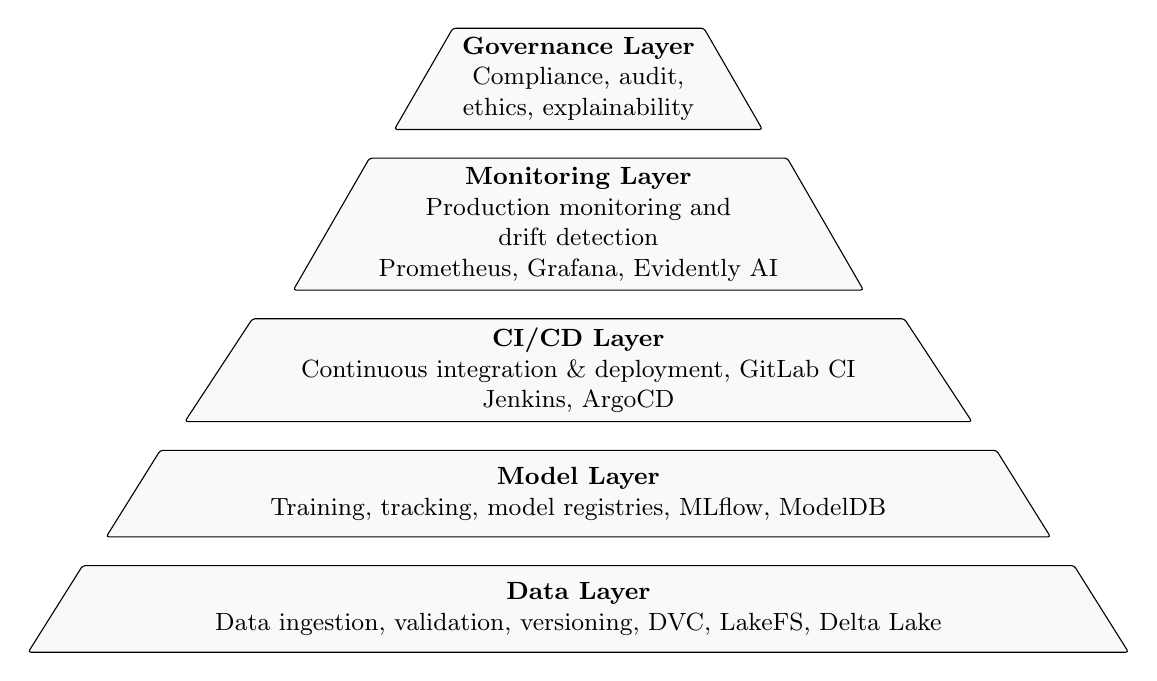
\begin{tikzpicture}[
		font=\small,
		layer/.style={
			trapezium,
			trapezium stretches=true,
			draw,
			rounded corners=1pt,
			align=center,
			minimum height=1.1cm,
			fill=gray!5
		}
		]
		
		% --- Data (base) ---
		\node[layer, minimum width=14cm] (data) {
			\textbf{Data Layer}\\
			Data ingestion, validation, versioning,
			DVC, LakeFS, Delta Lake
		};
		
		% --- Model ---
		\node[layer, minimum width=12cm, above=0.35cm of data] (model) {
			\textbf{Model Layer}\\
			Training, tracking, model registries, MLflow, ModelDB
		};
		
		% --- CI/CD ---
		\node[layer, minimum width=10cm, above=0.35cm of model] (cicd) {
			\textbf{CI/CD Layer}\\
			Continuous integration \& deployment, GitLab CI \\ Jenkins, ArgoCD
		};
		
		% --- Monitoring ---
		\node[layer, minimum width=3cm, above=0.35cm of cicd] (monitoring) {
			\textbf{Monitoring Layer}\\
			Production monitoring and \\ drift detection\\
			Prometheus, Grafana, Evidently AI
		};
		
		% --- Governance (top) ---
		\node[layer, minimum width=4cm, above=0.35cm of monitoring] (gov) {
			\textbf{Governance Layer}\\
			Compliance, audit,\\
			ethics, explainability
		};
		
	\end{tikzpicture}
	\caption{Conceptual MLOps pyramid with interdependent layers from data management to governance.}
	\label{fig:2.1}
\end{figure}

Each layer builds upon the previous one, forming a hierarchy of reproducibility and automation — from raw data to responsible deployment. We will keep it in mind and dive deeper in the next part of current text to understand what the key principle of MLOps are.

%------------------------------------------------
\subsection{Key Principles of MLOps}
MLOps is driven by several foundational principles:

\subsubsection*{Reproducibility.}
Every experiment, dataset, model, and environment must be uniquely identifiable and reproducible at any time. This ensures scientific integrity and traceability.

\subsubsection*{Automation (Pipelines).}
Training, validation, and deployment steps should be automated via pipelines (Airflow, Kubeflow, Tekton). Manual intervention is minimized.

\subsubsection*{Version Control.}
Not only source code, but also data, model parameters, and configurations must be versioned. Git is extended by tools like DVC and MLflow registries.

\subsubsection*{Continuous Training (CT).}
Analogous to Continuous Integration in software, models are retrained continuously as new data becomes available, keeping them current with evolving environments.

\subsubsection*{Model Drift and Retraining.}
Deployed models degrade as data distributions shift (``drift''). MLOps integrates drift detection, monitoring, and automated retraining workflows. \\

While, I guess all points are intuitively understandable, but the \textit{Model Drift} isn't. In the next part we will shortly introduce this phenomena.  

\subsection{Model Drift and Automated Retraining}

Deployed machine learning models operate in non-stationary environments. While the training process assumes that the joint distribution 
\[
P_{\text{train}}(X,Y) \approx P_{\text{future}}(X,Y),
\]
this assumption breaks down as physical conditions, data acquisition processes, or system dynamics evolve over time. \\

Such changes lead to \textbf{\emph{Model Drift}}, i.e., a degradation of predictive performance and physical consistency if no corrective mechanisms are introduced.


\subsubsection*{Types of Drift}

Model degradation can be categorized into three fundamental drift classes: \\

\begin{itemize}
	\item \textbf{Data Drift (Covariate Shift):}  
	The marginal input distribution changes while the underlying mapping remains stable:
	\[
	P_{\text{train}}(X) \neq P_{\text{live}}(X), \quad P(Y \mid X) \approx \text{const}.
	\]
	This can be detected using statistical divergence measures such as the Kolmogorov–Smirnov test, Population Stability Index (PSI), or Wasserstein distance.
	
	\item \textbf{Concept Drift:}  
	The conditional distribution changes:
	\[
	P_{\text{train}}(Y \mid X) \neq P_{\text{live}}(Y \mid X),
	\]
	which may occur in physical systems due to material aging, changing system dynamics, or updated operational conditions.
	
	\item \textbf{Model Drift:}  
	Even if the environment is stable, the model may become miscalibrated or insufficient due to limited capacity, dataset bias, or evolving rare events. \\
\end{itemize}

This overview should be enough to get the idea behind Model Drift, for more deeply information see the chapter \ref{cha:7}.

\section*{Summary}

In the context of this work, MLOps bridges the gap between experimental machine learning research and production-grade machine Learning systems.  
It introduces a rigorous lifecycle based on versioned data, tracked experiments, automated pipelines, continuously monitored deployments, and governed model operation. \\

Beyond the conceptual illustration of MLOps, the current work is accompanied by a concrete example derived from my master’s thesis. 
The objective of that thesis was to develop a machine learning procedure for solving an \textit{inverse heat conduction problem}, specifically to estimate a \textit{spatially dependent thermal diffusivity field}. 
In this work, this approach is extended into an MLOps context, with the goal of designing a production-capable system for predicting thermal diffusivity using automated and reproducible machine learning workflows. \\

In the context of machine learning for physical system modeling, several approaches exist. 
One particularly relevant method is the class of \textit{Physics-Informed Neural Networks} (PINNs). 
During my thesis, I developed a PINN to solve the above-mentioned inverse heat problem. 
This method and its theoretical foundation will be briefly introduced in the following section.


\section{Example: Scientific Machine Learning (PINNs)}

To illustrate, consider the inverse heat conduction problem:
\[
\partial_t u - \nabla \cdot (a(x,y)\nabla u) = f(x,y,t),
\]
where the goal is to infer the spatially varying diffusivity \(a(x,y)\) and possibly the source term \(f(x,y,t)\) from observed temperature data \(u(x,y,t)\).\\

The developed PINN system can be summarized as it is done in figure \ref{fig:2.2}. If some is more interested in details of my work please see \cite{Gesler_2025}. But for the terms of ML the Loss equations are important should be introduced here:

\begin{align}
	\mathcal{L}_{u_\text{D}} = \frac{1}{m} \| \hat{u}_l - u_D\|^2_2   \\
	\mathcal{L}_{f_\text{D}} = \frac{1}{m} \| \hat{f}_l - f_D \|^2_2
\end{align}

The above loss functions are used to train the models for the temperature $u$ and/or heat source $f$. Using them the main loss function for PINN can be calculated:

\begin{align}
	\mathcal{L}_{PDE} = \frac{1}{n}\| (\Tilde{u}_l)_t - \langle \nabla, \Tilde{a} \nabla \Tilde{u}\rangle - \Tilde{f} \|_{2}^{2}
\end{align}

That concludes this short introduction to the accompanying example. It is sufficient to assume that there exist some \hyperlink{https://github.com/RadmirG/Master-Arbeit}{\textbf{code sources}} that can be used as a basis and integrated into the MLOps system. The MLOps system will be designed to accept and analyze the measured data, to train the PINN, to use prediction to generate values and to monitor the reached results and PINN itself. The MLOps system will be derived step by step according to the chapters of this work. But firstly we will take a look how the PINN looks like in raw state as it now is and how it will be after the MLOps system is developed: \\

\textbf{Without MLOps} \\

\begin{itemize}
	\item Data preprocessing, network training, and validation occur manually.
	\item Each retraining (e.g., when new measurements arrive) requires manual repetition.
	\item No model versioning or metadata tracking — results are difficult to reproduce. \\
\end{itemize}

\textbf{With MLOps} \\

\begin{itemize}
	\item \textbf{Data Ingestion:} Experimental measurements are automatically collected and versioned (e.g., via DVC).
	\item \textbf{Training Pipeline:} Airflow triggers a PyTorch/DeepXDE training job on GPUs, logging all metrics to MLflow.
	\item \textbf{Model Registry:} The trained PINN is stored with version and metadata.
	\item \textbf{Deployment:} The model is deployed as an API service (e.g., KServe or FastAPI) for simulation queries.
	\item \textbf{Monitoring:} Drift detectors compare new observations with model predictions.
	\item \textbf{Retraining:} A CI/CD trigger starts retraining when deviation exceeds a threshold. \\
\end{itemize}

This workflow transforms a research prototype into a maintainable scientific software system — reproducible, observable, and scalable.

\begin{figure}[h]
	\centering       
	\begin{tikzpicture}[node distance=0.8cm and 0.8cm,
		ell/.style={draw, ellipse, minimum width=0.5cm, minimum height=0.5cm, fill=blue!5},
		forward/.style={->, dashed, gray}]		
		% ---------------------------------------------------------------------------------------
		% INPUT-LAYER
		% ---------------------------------------------------------------------------------------
		\node[ell] (data) {$\hat{\Omega} \times \hat{T}$};
		\node[ell, below=of data, yshift=0.5cm] (fD) {$f_D$};
		\node[ell, below=of fD, yshift=0.5cm] (uD) {$u_D$};
		\node[draw, dashed, rounded corners, fit=(fD) (data) (uD), inner sep=0.2cm, color=YellowGreen] (data_groupbox) {};
		
		\node[ell, below=of data_groupbox] (input) {$\Tilde{\Omega} \times \Tilde{T}$};
		% ---------------------------------------------------------------------------------------
		% NN FOR f(x)
		% ---------------------------------------------------------------------------------------
		\node[block, right=of input, xshift=1cm, yshift=4cm] (nn_f) {NN : $f_l(x,t)$};
		\node[block, below=of nn_f, xshift=1cm] (bpg_f) {$W_f = W'_f - \lambda \nabla_{W'_f} \mathcal{L}_{f_D}$};
		\node[block, right=of nn_f] (loss_f) {$\mathcal{L}_{f_D}$};
		\node[draw, dashed, rounded corners, fit=(nn_f) (bpg_f) (loss_f), inner sep=0.4cm] (groupbox_f) {};
		% Arrows		
		\draw[arrow, color=YellowGreen] (fD.east) 
		-- ([xshift=1cm]fD.east)
		-- ([xshift=1cm, yshift=-1.73cm]fD.east)
		-- ([xshift=6.7cm, yshift=-1.73cm]fD.east)
		-- ([xshift=6.7cm, yshift=1.125cm]fD.east)
		-- (loss_f.east);
		\draw[arrow] (nn_f) -- (loss_f);
		\draw[arrow] (loss_f) -- (bpg_f);
		\draw[arrow] (bpg_f) -- (nn_f);
		\draw[arrow, color=YellowGreen] (data) -- (nn_f);		
		% ---------------------------------------------------------------------------------------
		% NN FOR u(x)
		% ---------------------------------------------------------------------------------------
		\node[block, right=of input, xshift=1cm] (nn_u) {NN : $u_l(x,t)$};
		\node[block, below=of nn_u, xshift=1cm] (bpg_u) {$W_f = W'_f - \lambda \nabla_{W'_u} \mathcal{L}_{u_D}$};
		\node[block, right=of nn_u] (loss_u) {$\mathcal{L}_{u_D}$};
		\node[draw, dashed, rounded corners, fit=(nn_u) (bpg_u) (loss_u), inner sep=0.4cm] (groupbox_u) {};
		% Arrows
		\draw[arrow, color=YellowGreen] (uD.east) 
		-- ([xshift=0.8cm]uD.east)
		-- ([xshift=-4.82cm, yshift=0.5cm]loss_u.north)
		-- ([yshift=0.5cm]loss_u.north)
		-- (loss_u.north);	
		\draw[arrow] (nn_u) -- (loss_u);
		\draw[arrow] (loss_u) -- (bpg_u);
		\draw[arrow] (bpg_u) -- (nn_u);
		\draw[arrow,  color=YellowGreen] (data.west) 
		-- ([xshift=-0.4cm]data.west) 
		-- ([xshift=-4.018cm, yshift=1cm]nn_u.west) 
		-- ([xshift=-2cm, yshift=1cm]nn_u.west)
		-- (nn_u);
		% ---------------------------------------------------------------------------------------
		% PINN FOR a(x)
		% ---------------------------------------------------------------------------------------
		\node[block, right=of input, xshift=1.455cm, yshift=-4cm] (pinn_a) {PINN : $a_l(x)$};
		\node[block, right=of pinn_a, xshift=0.8cm] (AD) {AD};
		\node[block, right=of AD] (diff) {$(\Tilde{u}_l)_t, \langle \nabla, \Tilde{a}_l \nabla \Tilde{u} \rangle$};
		\node[block, below=of pinn_a] (bpg) {$W = W' - \lambda \nabla_{W'} \mathcal{L}$};
		\node[block, right=of bpg] (loss_a) {$\mathcal{L} = \mathcal{L}_{PDE}$};
		\node[draw, dashed, rounded corners, fit=(pinn_a) (diff) (bpg) (loss_a), inner sep=0.4cm] (groupbox_a) {};	
		\node[draw, circle, fill=blue!5, left=of pinn_a, xshift=-0.48cm] (x) {$x$};
		\node[draw, circle, fill=blue!5, above=of x, yshift=-0.8cm] (t) {$t$};
		% Arrows
		\draw[arrow, color=YellowGreen] ([yshift=-4cm]input.north) 
		-- (t) 
		-- ([xshift=8.2cm]t.east)
		-- (diff.north);
		\draw[arrow] (input.south) 
		-- ([yshift=-4cm]input.north)
		-- (x)
		-- (pinn_a.west);
		\draw[arrow] (pinn_a) -- (AD);
		\draw[arrow] (AD) -- (diff);
		\draw[arrow] (diff) -- (loss_a);
		\draw[arrow] (loss_a) -- (bpg);
		\draw[arrow] (bpg) -- (pinn_a);
		% ---------------------------------------------------------------------------------------
		% MODELS USE
		% ---------------------------------------------------------------------------------------	
		\node[right=of groupbox_f, xshift=0.6cm, yshift=1cm] (use_models) {Use as models};
		\node[ell, right=of groupbox_f, xshift=1cm] (model_f) {$f_l(x, t)$};
		\node[ell, right=of groupbox_u, xshift=1cm] (model_u) {$u_l(x, t)$};
		\draw [thick, decorate, decoration={brace,amplitude=12pt}] ([xshift=2.7cm]groupbox_f.north) -- ([xshift=2.7cm]groupbox_f.south) {};
		\draw [thick, decorate, decoration={brace,amplitude=12pt}] ([xshift=2.7cm]groupbox_u.north) -- ([xshift=2.7cm]groupbox_u.south) {};			
		% Arrows
		\draw[arrow] (input.south) 
		-- ([yshift=-3.35cm]input.north)
		-- ([xshift=8cm, yshift=-3.35cm]input.north)
		-- ([xshift=8cm, yshift=2.625cm]input.north)
		-- (model_f);	
		\draw[arrow] (input.south) 
		-- ([yshift=-3.35cm]input.north)
		-- ([xshift=8cm, yshift=-3.35cm]input.north)
		-- ([xshift=8cm, yshift=-1.35cm]input.north)
		-- (model_u);
		\draw[arrow] (model_u) -- (AD);
		\draw[arrow] (model_f.east) 
		-- ([xshift=1.15cm]model_f.east)
		-- ([xshift=1.15cm, yshift=-8.89cm]model_f.east)
		-- (loss_a.east);						
		\node[draw, dashed, rounded corners, fit=(use_models) (model_f) (model_u) , inner sep=0.2cm] (group_models) {};		
		% ---------------------------------------------------------------------------------------	
		\node[draw, rounded corners, fit=(groupbox_f) (groupbox_a) (groupbox_u) , inner sep=0.4cm] (groupbox) {};		
	\end{tikzpicture}
	\caption[Separated training of the PINN for the inverse heat conduction problem]{Separated training of the Physics-Informed Neural Network (PINN) for the inverse heat conduction problem with respect to thermal diffusivity.
		The neural networks for $u_l$ and $f_l$ are trained in independent training loops using the datasets $\hat{\Omega} \times \hat{T}$ and the measurement data $f_D$ and $u_D$, respectively.
		After this pretraining phase, the actual PINN training is carried out on the dataset $\tilde{\Omega} \times \tilde{T}$, where the pretrained models $u_l$ and $f_l$ are used to compute the PDE residual.
		The PINN itself receives only spatial inputs from $\tilde{\Omega}$.
		The green arrow originating from the node $t$ represents the temporal consistency of the training data and supplies the corresponding time values required for evaluating the derivatives of $u_l$.}
	
	\label{fig:2.2}
\end{figure}




	\chapter{Core MLOps Architecture}

The objective of this module is to understand how the core components of an MLOps ecosystem fit together, and how containerization, orchestration, and automation form the foundation of scalable, reproducible machine learning systems.  
We will explore the relationship between \textbf{Docker}, \textbf{Kubernetes}, and \textbf{OpenShift} as infrastructural layers, and how these integrate with higher-level ML services such as \textbf{Airflow}, \textbf{MLflow}, and \textbf{Kubeflow}.

%------------------------------------------------
\section*{Stack Overview}
At the heart of modern MLOps lies the idea of \textbf{infrastructure abstraction}: machine learning workloads are encapsulated inside containers and orchestrated across clusters in a reproducible and portable manner.  
A typical stack can be described as follows:
\begin{itemize}[leftmargin=1.5cm]
	\item \textbf{Docker + Kubernetes} provide environment isolation, scalability, and infrastructure abstraction.
	\item \textbf{Airflow}, \textbf{Kubeflow}, and \textbf{MLflow} integrate to deliver automation, tracking, and governance.
	\item \textbf{Declarative Pipelines} (YAML/JSON, Argo, Tekton) define reproducible workflows as code.
	\item \textbf{GitOps} principles ensure versioned, auditable, and automatically deployed infrastructure.
\end{itemize}

These layers work together to move from experimentation to production while maintaining scientific rigor, operational stability, and continuous improvement.

%------------------------------------------------
\section*{From Containers to Clusters: Docker, Kubernetes, and OpenShift}

\subsection*{Docker: The Fundamental Building Block}
\textbf{Docker} provides a lightweight mechanism to package applications, dependencies, and environments into isolated \textit{containers}.  
A Docker container behaves like a minimal operating system containing exactly what the program needs to run, ensuring consistent behavior across development, testing, and production.

\subsection*{Conceptual analogy:}
Each container is like a \textit{single laboratory box}—self-contained, portable, and isolated.  
It has:
\begin{itemize}
	\item Its own filesystem (based on the Docker image).
	\item Its own process space and networking.
	\item Shared access to the host’s Linux kernel.
\end{itemize}

\subsection*{Why this matters for MLOps:}
Reproducibility is central to scientific ML.  
A Docker container guarantees that a trained model behaves identically whether it runs on a local workstation, a GPU server, or a cloud node.

\subsection*{Example:}
\begin{verbatim}
docker build -t pinn-trainer .
docker run --gpus all -v ./data:/data pinn-trainer
\end{verbatim}
This command builds and launches a reproducible environment to train a Physics-Informed Neural Network (PINN) on GPU hardware.

\subsection*{Docker Compose: Managing Multiple Containers}
As soon as an ML workflow involves multiple services—such as a training script, a database, and a monitoring dashboard—\textbf{Docker Compose} provides a unified configuration layer.

\subsection*{Example:}
\begin{verbatim}
services:
  mlflow:
    image: ghcr.io/mlflow/mlflow:v2.16.0
    ports: ["5000:5000"]
  postgres:
    image: postgres:15
    environment:
      POSTGRES_PASSWORD: example
\end{verbatim}

Compose simplifies orchestration on a single machine, but it remains limited to one host.

\subsection*{Kubernetes: Orchestrating Containers Across Clusters}
When workloads must scale across multiple machines, \textbf{Kubernetes (K8s)} acts as an \textit{orchestrator}.  
It automatically deploys, scales, and monitors containers across a distributed cluster of nodes.

\subsection*{Key Kubernetes concepts:}
\begin{itemize}
	\item \textbf{Pod:} Smallest deployable unit (one or more containers).
	\item \textbf{Node:} A physical or virtual machine where Pods run.
	\item \textbf{Deployment:} Blueprint for desired number of replicas and version management.
	\item \textbf{Service:} Provides a stable network endpoint for distributed Pods.
	\item \textbf{Ingress:} Manages external access (HTTP/HTTPS routing).
\end{itemize}

Kubernetes ensures high availability, self-healing, and dynamic scaling, forming the operational core of most MLOps infrastructures.

\subsection*{Analogy:}
If each Docker container is a \textit{laboratory box}, Kubernetes is the \textit{facility manager}—it allocates space, restarts failed experiments, and keeps the environment balanced.

\subsection*{OpenShift: The Enterprise Platform Layer}
\textbf{OpenShift} is Red Hat’s enterprise-grade platform built on top of Kubernetes.  
It provides a more opinionated, secure, and user-friendly ecosystem by integrating:
\begin{itemize}
	\item Developer tooling (builds, web console, source-to-image).
	\item CI/CD (Tekton pipelines, ArgoCD).
	\item Security and governance (OAuth, RBAC, quotas).
	\item Monitoring and logging (Prometheus, Grafana, EFK).
\end{itemize}

\subsection*{Analogy:}
Kubernetes is the engine; OpenShift is the fully assembled car with integrated dashboards, autopilot, and safety systems.

\subsection*{Architectural Layering:}
\begin{center}
     \begin{verbatim}
                    |-------------------------------|
                    | OpenShift (Platform Layer)    |
                    |  |-- Developer Tools, CI/CD   |
                    |  |-- Security, Monitoring     |
                    |--------------|----------------|
                                   |
                    |--------------|----------------|
                    | Kubernetes (Orchestration)    |
                    |  |-- Pods, Deployments, Nodes |
                    |  |-- Services, Ingress        |
                    |--------------|----------------|
                                   |
                    |--------------|----------------|
                    | Docker / CRI-O (Runtime)      |
                    |  |-- Images, Containers       |
                    |--------------|----------------|
                                   |
                    |--------------|----------------|
                    | Host OS (e.g., Ubuntu)        |
                    |-------------------------------|
    \end{verbatim}
\end{center}

This stack provides a full abstraction from hardware to application-level MLOps orchestration.

%------------------------------------------------
\section*{Architecture Layout}

An MLOps system can be conceptualized as multiple layers, from infrastructure to model governance:

\begin{verbatim}
+-----------------------------------------------------------+
|               Model Governance & Monitoring               |
|      (Evidently, Prometheus, Grafana, WhyLabs, etc.)      |
+-----------------------------------------------------------+
|                   Continuous Deployment                   |
|    (ArgoCD, Jenkins, GitLab CI/CD, Tekton Pipelines)      |
+-----------------------------------------------------------+
|             ML Workflow Orchestration Layer               |
| (Airflow, Kubeflow Pipelines, Prefect, Dagster, etc.)     |
+-----------------------------------------------------------+
|            Experiment Tracking & Model Registry           |
|                   (MLflow, ModelDB)                       |
+-----------------------------------------------------------+
|                 Containerized Training                    |
|            (Docker, Kubernetes, OpenShift)                |
+-----------------------------------------------------------+
|              Data Versioning and Ingestion                |
|           (DVC, LakeFS, Delta Lake, Feast)                |
+-----------------------------------------------------------+
|                     Hardware Layer                        |
|              (CPU, GPU, TPU clusters, Cloud)              |
+-----------------------------------------------------------+
\end{verbatim}

Each layer can evolve independently but interacts via versioned interfaces and declarative specifications.

%------------------------------------------------
\section*{Discussion}

\subsection*{Why Kubernetes/OpenShift Forms the Backbone.}
Kubernetes abstracts away infrastructure complexity. It treats compute nodes as a uniform resource pool, automatically managing container scheduling, scaling, and failover.  
OpenShift extends this with enterprise features—security, governance, multi-tenancy—making it suitable for research labs, production environments, and hybrid cloud deployments.

\subsection*{Containerization as a Reproducibility Mechanism.}
Every experiment or training run can be encapsulated into a container image, ensuring identical results across hardware or environments.  
This property is critical in scientific ML, where reproducibility is as important as accuracy.

\subsection*{CI/CD and Infrastructure-as-Code Integration.}
MLOps inherits from DevOps the principles of automation and version control:
\begin{itemize}
	\item \textbf{CI (Continuous Integration)} ensures that code changes are tested and validated automatically.
	\item \textbf{CD (Continuous Deployment)} enables fast, safe delivery of new models and services.
	\item \textbf{Infrastructure as Code (IaC)} expresses the entire system (nodes, pods, services, pipelines) as declarative YAML or JSON—enabling complete environment recreation.
\end{itemize}

Together, these mechanisms make ML systems scalable, observable, and maintainable—transforming one-time experiments into continuously evolving, production-grade scientific platforms.


%------------------------------------------------
\section{Airflow, Kubeflow, and MLflow: Integration Patterns}

\subsection*{Roles and Interfaces}
\begin{itemize}[leftmargin=1.5cm]
  \item \textbf{Airflow} orchestrates the \emph{end-to-end workflow}: data ingestion, validation, triggering training, post-processing, and deployment gates. It is task-centric and environment-agnostic.
  \item \textbf{Kubeflow (Pipelines + Katib + KServe)} executes \emph{ML-specific jobs} on Kubernetes/OpenShift: GPU training, hyperparameter tuning, and model serving with autoscaling.
  \item \textbf{MLflow} provides \emph{experiment tracking} and a \emph{model registry}: parameters, metrics, artifacts, and model versions for governance and rollbacks.
\end{itemize}

\subsection{Data Flow.} Airflow triggers a Kubeflow Pipeline (KFP) step that runs the GPU training container for the PINN. That step logs parameters/metrics/artifacts to MLflow. After evaluation, Airflow promotes the best run into the MLflow Model Registry and triggers a KServe deployment from the registered artifact.

%------------------------------------------------
\subsection*{End-to-end PINN Example (Research $\rightarrow$ Production)}
Suppose we have:
\begin{itemize}
  \item \texttt{pinn\_model.py} defining \(u_\theta(x,y,t)\), PDE residuals, and loss terms.
  \item \texttt{train.py} training the PINN on GPUs and logging to MLflow.
  \item \texttt{serve.py} (optional) packing a prediction endpoint for offline serving.
\end{itemize}

\subsection*{Airflow DAG (high-level).}
\begin{verbatim}
@dag(schedule_interval="@daily", catchup=False)
def inverse_heat_mlops():
    prepare_data()     # ETL, validation, dataset versioning
    run_kfp_training() # trigger Kubeflow Pipeline job on GPU
    evaluate_runs()    # pick best MLflow run by metric (e.g., PDE residual)
    register_model()   # promote to MLflow Model Registry (stage="Staging")
    deploy_kserve()    # rolling deploy via KServe from the Registry artifact
\end{verbatim}

\subsection*{Kubeflow Pipeline step (pseudo-spec).}
\begin{verbatim}
component:
  name: Train PINN
  inputs: [dataset_uri, mlflow_uri, epochs, lr, a_reg, f_reg]
  container:
    image: registry/app/pinn-trainer:latest
    command:
      - python
      - /app/train.py
      - --data={{inputs.dataset_uri}}
      - --epochs={{inputs.epochs}}
      - --lr={{inputs.lr}}
      - --mlflow={{inputs.mlflow_uri}}
      - --a-reg={{inputs.a_reg}}
      - --f-reg={{inputs.f_reg}}
    resources:
      limits: {nvidia.com/gpu: "1"}
\end{verbatim}

\subsection*{MLflow logging within \texttt{train.py} (excerpt).}
\begin{verbatim}
import mlflow, mlflow.pytorch as mpt
mlflow.set_tracking_uri(os.environ.get("MLFLOW_TRACKING_URI"))
mlflow.set_experiment("inverse-heat-pinn")

with mlflow.start_run(run_name="pinn-gpu"):
    mlflow.log_param("epochs", epochs)
    mlflow.log_param("lr", lr)
    mlflow.log_param("a_reg", a_reg)
    mlflow.log_param("f_reg", f_reg)
    # ... training loop; log losses and PDE residuals
    mlflow.log_metric("train_residual", residual_value, step=epoch)
    # save model + artifacts (e.g., plots, checkpoints)
    mpt.log_model(model, artifact_path="model")
\end{verbatim}

\subsection*{Promotion \& deployment gate.} After training completes, a gate task in Airflow queries MLflow for the best run (e.g., minimal PDE residual or validation error). If thresholds are met, Airflow:
\begin{enumerate}
  \item Promotes the run in the MLflow \emph{Model Registry} (e.g., from ``None'' to ``Staging'' or ``Production'').
  \item Triggers a \emph{KServe} deployment pulling the artifact from the Registry storage (PVC/S3).
\end{enumerate}

%------------------------------------------------
\section*{Declarative Pipelines (YAML/JSON, Argo, Tekton)}
MLOps pipelines should be \emph{infrastructure-as-code}. Declarative specs ensure repeatability, reviews, and auditability.

\subsection*{Examples}
\subsection*{Argo Workflow snippet (conceptual).}
\begin{verbatim}
apiVersion: argoproj.io/v1alpha1
kind: Workflow
metadata: { name: inverse-heat-pinn }
spec:
  entrypoint: main
  templates:
  - name: main
    steps:
    - - name: etl
        template: etl
      - name: train
        template: train
      - name: evaluate
        template: evaluate
      - name: deploy
        template: deploy
  - name: train
    container:
      image: registry/app/pinn-trainer:latest
      command: ["python","/app/train.py","--mlflow=http://mlflow:5000"]
\end{verbatim}

\subsection*{Tekton Pipeline snippet (OpenShift Pipelines).}
\begin{verbatim}
apiVersion: tekton.dev/v1
kind: Pipeline
metadata: { name: pinn-train-deploy }
spec:
  tasks:
  - name: train
    taskRef: { name: python-task }
    params:
    - name: image
      value: registry/app/pinn-trainer:latest
    - name: args
      value:
      - python
      - /app/train.py
      - --mlflow=$(params.mlflow_uri)
  - name: deploy
    runAfter: ["train"]
    taskRef: { name: kserve-deploy-task }
\end{verbatim}

By storing these YAML specs in Git, we enable reviews, rollbacks, and reproducible automation across environments.

%------------------------------------------------
\section*{GitOps Principles}
\textbf{GitOps} manages both \emph{applications} and \emph{infrastructure} through Git as the single source of truth. A controller (e.g., Argo CD) reconciles the live cluster state to match the Git state.

\subsection*{Core Practices}
\begin{itemize}[leftmargin=1.5cm]
  \item Store Kubernetes/OpenShift manifests (Deployments, Services, Ingress/Routes, KServe, Tekton) in Git.
  \item Use branches/tags for \emph{environments} (e.g., \texttt{dev}, \texttt{staging}, \texttt{prod}).
  \item Rely on \emph{pull requests} for all changes (audit trail, review).
  \item Argo CD continuously compares live cluster state with Git and applies drifts back to the desired config.
\end{itemize}

\subsection*{Benefit for PINNs.}
Changes in PDE loss weights, architecture, or serving resources (e.g., GPUs, memory) are versioned and reviewed. Rollbacks are trivial, and experiments map cleanly to infrastructure changes.

%------------------------------------------------
\section*{How OpenShift Integrates with Airflow, Kubeflow, and MLflow}

\subsection*{OpenShift as the Enterprise Kubernetes Layer}
OpenShift provides:
\begin{itemize}[leftmargin=1.5cm]
  \item \textbf{Security \& Auth}: OAuth, RBAC, SCCs (Security Context Constraints).
  \item \textbf{Builds \& CI/CD}: OpenShift Pipelines (Tekton), OpenShift GitOps (Argo CD).
  \item \textbf{Registry \& Routes}: Integrated image registry and HTTP(S) routing via Routes.
  \item \textbf{Monitoring}: Prometheus/Grafana baked in; EFK for logs.
\end{itemize}

\subsection*{Running Airflow on OpenShift}
\begin{itemize}[leftmargin=1.5cm]
  \item Package Airflow components as Deployments (webserver, scheduler, workers) with a \texttt{ClusterIP} Service and an OpenShift \texttt{Route}.
  \item Workers can request GPUs (\texttt{nvidia.com/gpu}) if PINN training is executed inside Airflow tasks.
  \item Airflow tasks trigger Kubeflow Pipelines via KFP SDK or Argo/Tekton via API.
\end{itemize}

\subsection*{Airflow Deployment (conceptual).}
\begin{verbatim}
apiVersion: apps/v1
kind: Deployment
metadata: { name: airflow-worker }
spec:
  template:
    spec:
      containers:
      - name: worker
        image: registry/airflow:2.10
        resources:
          limits: { nvidia.com/gpu: "1" }
\end{verbatim}

\subsection*{Kubeflow / KServe on OpenShift}
\begin{itemize}[leftmargin=1.5cm]
  \item Use \textbf{KServe} to serve models from MLflow artifacts (PVC, S3, or object storage).
  \item Auto-scaling via Knative; traffic management via OpenShift Routes/Ingress.
\end{itemize}

\subsection*{KServe \texttt{InferenceService} for PINN (conceptual).}
\begin{verbatim}
apiVersion: serving.kserve.io/v1beta1
kind: InferenceService
metadata: { name: pinn-predictor }
spec:
  predictor:
    pytorch:
      storageUri: s3://mlflow-artifacts/inverse-heat-pinn/Production
      resources:
        limits: { nvidia.com/gpu: "1", cpu: "2", memory: "8Gi" }
\end{verbatim}

\subsection*{MLflow on OpenShift}
\begin{itemize}[leftmargin=1.5cm]
  \item Run MLflow as a Deployment with a PersistentVolumeClaim for \texttt{backend-store} (e.g., SQLite/PostgreSQL) and \texttt{artifact-store} (PVC/S3).
  \item Expose MLflow UI via an OpenShift \texttt{Route}.
\end{itemize}

\subsection*{MLflow Deployment (conceptual).}
\begin{verbatim}
apiVersion: apps/v1
kind: Deployment
metadata: { name: mlflow }
spec:
  template:
    spec:
      containers:
      - name: mlflow
        image: ghcr.io/mlflow/mlflow:v2.16.0
        args: ["mlflow","server","--host","0.0.0.0","--port","5000",
               "--backend-store-uri","postgresql://.../mlflow",
               "--default-artifact-root","s3://mlflow-artifacts/"]
\end{verbatim}

\subsection*{Putting It Together on OpenShift (GitOps)}
\begin{enumerate}
  \item \textbf{Git Repos}:
    \begin{itemize}
      \item \textit{App repo}: PINN code (\texttt{pinn\_model.py}, \texttt{train.py}, Dockerfile).
      \item \textit{Ops repo}: OpenShift/K8s manifests (Airflow, MLflow, KServe, Tekton Pipelines).
    \end{itemize}
  \item \textbf{Build \& Push}: OpenShift BuildConfigs or external CI build/push images to the internal registry.
  \item \textbf{Deploy via Argo CD}: Sync manifests in \textit{ops repo} to cluster namespaces (\texttt{dev} $\rightarrow$ \texttt{staging} $\rightarrow$ \texttt{prod}).
  \item \textbf{Run Pipeline}: Tekton or Argo executes the declarative pipeline (ETL $\rightarrow$ Train $\rightarrow$ Evaluate $\rightarrow$ Deploy).
  \item \textbf{Observe}: Prometheus/Grafana dashboards + MLflow metrics; alert on drift (Evidently) and trigger retraining.
\end{enumerate}

%------------------------------------------------
\section*{Operational Notes for the PINN Use Case}
\begin{itemize}[leftmargin=1.5cm]
  \item \textbf{Data versioning}: store measurement batches (HDF5/Parquet) with DVC/LakeFS; pass concrete dataset URIs into KFP runs.
  \item \textbf{Resource profiles}: declare GPU requests/limits per training task to ensure fair scheduling on shared clusters.
  \item \textbf{Artifacts}: save training curves, PDE residual maps, and mesh plots as MLflow artifacts to audit physical validity.
  \item \textbf{Promotion policy}: require thresholds on PDE residuals and boundary-condition violations before model promotion.
  \item \textbf{Rollback}: Argo CD and MLflow Registry both provide quick rollback to known-good model and manifests.
\end{itemize}

%------------------------------------------------
\section*{Summary (Integration at a Glance)}
\begin{itemize}[leftmargin=1.5cm]
  \item \textbf{Airflow} = orchestration of the end-to-end job graph (triggers KFP/Tekton).
  \item \textbf{Kubeflow} = GPU training, tuning (\emph{Katib}), and \emph{KServe} for serving.
  \item \textbf{MLflow} = experiment tracking + registry for PINN model governance.
  \item \textbf{Declarative Pipelines} = Argo/Tekton YAML encode the workflow as code.
  \item \textbf{GitOps} = Argo CD keeps the cluster aligned with Git manifests.
  \item \textbf{OpenShift} = enterprise Kubernetes with security, routes, registry, pipelines, and GitOps—hosting all components consistently.
\end{itemize}

	\chapter{Data and Experiment Management}

\section*{Goal}
The goal of this module is to design a reproducible strategy for handling data, experiments, and models throughout the machine learning lifecycle.  
In scientific ML, this step ensures that datasets, scripts, and results can be precisely reproduced, verified, and compared across iterations.  
Reproducibility is not only an engineering necessity but also a scientific requirement.

%------------------------------------------------
\section*{Conceptual Overview}
Every experiment can be expressed as a tuple:
\[
E = (\mathcal{D}, \mathcal{M}, \Theta, \mathcal{R}),
\]
where
\begin{itemize}
	\item \(\mathcal{D}\) — dataset or measurement configuration,
	\item \(\mathcal{M}\) — model architecture and implementation,
	\item \(\Theta\) — hyperparameters and physical constants,
	\item \(\mathcal{R}\) — results (metrics, residuals, and artifacts).
\end{itemize}
Managing experiments therefore requires version control over all components of \(E\).  
Tools such as DVC, LakeFS, Feast, and MLflow provide complementary functionality within this framework.

%------------------------------------------------
\section*{Data Versioning}
Reproducible research demands that the dataset used for each training run can be reconstructed exactly — down to preprocessing and filtering steps.  
This is especially critical when dealing with measurement noise, temporal drift, or simulation snapshots in PDE data.

\subsection*{DVC (Data Version Control)}
\textbf{DVC} extends Git semantics to large datasets.  
Instead of storing data directly in the repository, it creates lightweight \texttt{.dvc} metafiles containing hashes and remote storage references.

\subsection*{Typical workflow:}
\begin{verbatim}
dvc init
dvc remote add origin s3://research-datasets
dvc add data/measurements.h5
git add data/measurements.h5.dvc .gitignore
git commit -m "Add initial measurement dataset"
dvc push
\end{verbatim}

This guarantees that any model training job can reproduce the exact dataset version simply by:
\begin{verbatim}
dvc pull
\end{verbatim}

\subsection*{Integration into the PINN pipeline:}
Each Airflow/Kubeflow training step begins by running \texttt{dvc pull} to fetch the correct version of \(u(x,y,t)\) measurements before training the inverse heat model.  
The DVC hash is logged into MLflow as a \texttt{data\_version} parameter for full lineage tracking.

\subsection*{LakeFS}
\textbf{LakeFS} provides Git-like version control for large-scale object storage (S3, GCS, Azure).  
It allows creation of isolated data branches for experiments, enabling parallel workflows:
\begin{itemize}
	\item \texttt{main} branch for stable, validated datasets.
	\item \texttt{exp/\#42} branch for experimental preprocessing or noise filtering.
\end{itemize}
When an experiment finishes, the branch can be merged into \texttt{main} or discarded.

\subsection*{Example:}
The research team can branch the raw thermal measurement data into \texttt{exp/pinn-filtered} for preprocessing with spatial smoothing before training the PINN.  
This ensures that the original raw data remains untouched and fully recoverable.

%------------------------------------------------
\section*{Feature Stores}
While DVC and LakeFS handle raw datasets, a \textbf{Feature Store} centralizes precomputed features for model consumption.  
This is crucial for production models that must ensure feature consistency between training and inference.

\subsection*{Feast}
\textbf{Feast} (Feature Store) provides:
\begin{itemize}
	\item Central registry of feature definitions (e.g., averaged heat flux, boundary gradients).
	\item Offline store (for training) and online store (for inference) synchronization.
	\item Consistent versioning and timestamps.
\end{itemize}

\subsection*{Example:}
In the PINN inverse heat workflow, precomputed features such as
\[
\phi_1(x,y) = \nabla_x u(x,y,t), \quad
\phi_2(x,y) = \nabla_y u(x,y,t)
\]
can be stored in Feast for reuse across experiments with different boundary conditions.  
The same features are available both to the training container and to real-time simulations served by KServe.

%------------------------------------------------
\section*{Experiment Tracking with MLflow}
\textbf{MLflow} serves as the central hub for recording all metadata produced by training runs:
\begin{itemize}[leftmargin=1.5cm]
	\item \textbf{Parameters:} hyperparameters, regularization weights, learning rates.
	\item \textbf{Metrics:} losses, PDE residual norms, validation errors.
	\item \textbf{Artifacts:} model checkpoints, plots, configuration files.
	\item \textbf{Tags:} experiment identifiers, dataset versions, and domain parameters.
\end{itemize}

\subsection*{Example Logging Script.}
\begin{verbatim}
with mlflow.start_run(run_name="inverse-heat-a=xy-var"):
    mlflow.log_param("dataset_hash", dvc_hash)
    mlflow.log_param("architecture", "PINN-5x128")
    mlflow.log_param("a_reg", 1e-3)
    mlflow.log_metric("pde_loss", loss_pde)
    mlflow.log_metric("bc_loss", loss_bc)
    mlflow.log_metric("val_residual", residual_norm)
    mlflow.log_artifact("plots/residual_map.png")
\end{verbatim}

\subsection*{Model Registry.}
Trained models can be registered with metadata and version numbers:
\begin{verbatim}
mlflow.register_model(
    "runs:/<run_id>/model",
    "inverse-heat-pinn"
)
\end{verbatim}
Later stages of the MLOps pipeline (Airflow or Tekton) can promote models between stages (\texttt{Staging} → \texttt{Production}) based on performance metrics.

\subsection*{Structured Experimentation.}
Tags allow automatic grouping:
\begin{verbatim}
mlflow.set_tags({
    "domain": "heat-inverse",
    "dataset_branch": "exp/pinn-filtered",
    "equation": "u_t - div(a grad u) = f",
    "optimizer": "Adam"
})
\end{verbatim}

Experiments can then be queried or visualized via the MLflow UI or API, enabling comparisons across architectures and loss-weight configurations.

%------------------------------------------------
\section*{Model Lineage and Governance}
\textbf{Model lineage} traces the complete genealogy of a trained model:
\[
\text{Model} \rightarrow (\text{Code Version}, \text{Data Version}, \text{Parameters}, \text{Environment}).
\]
Governance extends this with policies for reproducibility, approval, and compliance.

\subsection*{In practice:}
\begin{itemize}
	\item \textbf{Code lineage:} captured via Git commit SHA and Docker image tag.
	\item \textbf{Data lineage:} captured via DVC or LakeFS dataset hashes.
	\item \textbf{Experiment lineage:} maintained via MLflow runs and registered model versions.
	\item \textbf{Model approval:} controlled via MLflow Registry stages and CI/CD policies.
\end{itemize}

\subsection*{Governance Workflow in the PINN Project.}
\begin{enumerate}
	\item Each training run logs its dataset version (\texttt{dvc hash}), source commit, and container image.
	\item Airflow automatically attaches these identifiers as MLflow tags.
	\item A Tekton or ArgoCD gate promotes models that satisfy physics and validation constraints.
	\item All promotions are versioned in GitOps repositories for auditability.
\end{enumerate}

%------------------------------------------------
\section*{Example: Tracking PINN Experiments for \( a(x,y) \)}
In the inverse heat problem
\[
\partial_t u - \nabla \cdot (a(x,y)\nabla u) = f(x,y,t),
\]
the goal is to infer both the thermal diffusivity \(a(x,y)\) and possibly \(f(x,y,t)\) from measured \(u(x,y,t)\).

\subsection*{Experiment setup.}
\begin{itemize}
	\item \textbf{Dataset:} generated from simulated or experimental temperature fields, versioned with DVC.
	\item \textbf{Model:} PINN architecture (\(u_\theta(x,y,t)\)) defined in \texttt{pinn\_model.py}.
	\item \textbf{Training Script:} \texttt{train.py}, parameterized by network depth, learning rate, and loss weights.
	\item \textbf{Tracking:} all runs logged to MLflow under the experiment \texttt{inverse-heat-pinn}.
\end{itemize}

\subsection*{Use Case.}
Different hypotheses for \(a(x,y)\) (e.g., polynomial vs.\ neural approximation) can be compared through their MLflow runs:
\begin{itemize}
	\item Runs grouped by tag \texttt{architecture}.
	\item Metrics such as PDE residual or boundary violation used for comparison.
	\item Results visualized as contour plots (logged as artifacts).
\end{itemize}

\subsection*{Outcome.}
By combining DVC (data versioning), LakeFS (branching datasets), Feast (feature management), and MLflow (experiment tracking), each PINN run is fully reproducible and scientifically auditable.  
This enables quantitative comparison of modeling choices, reliable peer verification, and compliant long-term archiving of simulation results.

	\chapter{Pipelines and Automation}

\section*{Goal}
The goal of this chapter is to design fully automated workflows that connect all components of the MLOps ecosystem --- from data ingestion to model deployment.  
Automation ensures that every experiment, retraining, and deployment follows a repeatable, versioned process without manual intervention.  
In the context of scientific ML, such automation also supports reproducibility, traceability, and continuous scientific improvement.

%------------------------------------------------
\section*{Motivation}
Machine learning pipelines are often complex, involving data validation, model training, evaluation, and deployment across heterogeneous systems.  
Manual orchestration is error-prone, difficult to reproduce, and does not scale.  
Automated pipelines encapsulate this complexity into declarative, executable workflows.

A well-designed MLOps pipeline transforms an idea into a measurable experiment:
\[
\text{Data Ingestion} \rightarrow \text{Training} \rightarrow \text{Evaluation} \rightarrow \text{Deployment} \rightarrow \text{Monitoring}.
\]

These steps form a continuous feedback loop for improving both model accuracy and operational robustness.

%------------------------------------------------
\section*{Tools and Orchestration Layers}
Automation in MLOps typically involves multiple layers of orchestration:

\subsection*{Airflow DAGs (Directed Acyclic Graphs)}
\textbf{Apache Airflow} is a general-purpose workflow orchestrator.  
It defines pipelines as DAGs where each node represents a task (e.g., data preprocessing, training, evaluation).  
Airflow provides:
\begin{itemize}[leftmargin=1.5cm]
	\item Python-based pipeline definition.
	\item Rich scheduling and dependency management.
	\item Integration with Kubernetes and external services.
	\item Fine-grained monitoring through the Airflow Web UI.
\end{itemize}

\subsection{Conceptual Role.}
Airflow is the high-level \emph{conductor} coordinating the entire workflow.  
It can trigger Kubeflow Pipelines, Tekton pipelines, or even shell scripts for specialized tasks.

\subsection*{Kubeflow Pipelines}
\textbf{Kubeflow Pipelines (KFP)} run machine learning tasks natively on Kubernetes/OpenShift.  
Each step in a pipeline is a containerized component, ensuring reproducibility and scalability.

\subsection{Capabilities.}
\begin{itemize}[leftmargin=1.5cm]
	\item Parameterized training and hyperparameter tuning.
	\item Distributed GPU/CPU scheduling.
	\item Integration with MLflow, S3, or MinIO artifact storage.
	\item Execution history with visualization of DAGs and metrics.
\end{itemize}

In the context of the inverse heat problem, a Kubeflow Pipeline might include:
\begin{enumerate}
	\item Fetching and validating temperature datasets.
	\item Launching the PINN training container on GPU nodes.
	\item Logging metrics and residuals to MLflow.
	\item Evaluating physics-based losses.
	\item Registering the best-performing model.
\end{enumerate}

\subsection*{Tekton / Argo Workflows}
\textbf{Tekton} (OpenShift Pipelines) and \textbf{Argo Workflows} implement pipelines declaratively using YAML or JSON specifications.

\subsection{Advantages.}
\begin{itemize}[leftmargin=1.5cm]
	\item Pipelines are stored in Git --- enabling versioned, auditable, and declarative automation (GitOps).
	\item Each task runs as a Kubernetes Pod, scaling automatically.
	\item Seamless integration with CI/CD systems (e.g., GitLab or Jenkins).
\end{itemize}

\subsection{Example:}
A Tekton pipeline in OpenShift could express the same PINN training workflow as a sequence of tasks:
\begin{verbatim}
apiVersion: tekton.dev/v1
kind: Pipeline
metadata:
  name: inverse-heat-pinn
spec:
  tasks:
  - name: fetch-data
    taskRef: { name: dvc-fetch }
  - name: train
    runAfter: ["fetch-data"]
    taskRef: { name: pinn-train }
  - name: evaluate
    runAfter: ["train"]
    taskRef: { name: evaluate-metrics }
  - name: register
    runAfter: ["evaluate"]
    taskRef: { name: mlflow-register }
  - name: deploy
    runAfter: ["register"]
    taskRef: { name: kserve-deploy }
\end{verbatim}

\subsection{Execution Context.}
Each task in this pipeline runs in an isolated container with its own resource request (e.g., GPU, CPU, memory).  
This separation ensures reproducibility and efficient utilization of compute clusters.

%------------------------------------------------
\section*{Automated Retraining and Evaluation}
Scientific ML systems often operate on time-dependent or evolving data.  
Automated retraining ensures that the model remains accurate and consistent as new observations are collected.

\subsection{Triggering mechanisms.}
\begin{itemize}[leftmargin=1.5cm]
	\item \textbf{Time-based retraining:} Airflow schedules a pipeline (e.g., daily or weekly).
	\item \textbf{Event-based retraining:} A new dataset commit (DVC push or LakeFS merge) triggers Tekton/Argo.
	\item \textbf{Drift-based retraining:} Monitoring systems (Evidently AI or Prometheus alerts) detect data or model drift and trigger retraining automatically.
\end{itemize}

\subsection{Evaluation.}
Every retraining run is evaluated using both statistical and physical metrics:
\[
\mathcal{L}_{\text{total}} = w_{\text{PDE}}\mathcal{L}_{\text{PDE}} + 
w_{\text{BC}}\mathcal{L}_{\text{BC}} + 
w_{\text{IC}}\mathcal{L}_{\text{IC}}.
\]
Metrics are logged in MLflow and visualized in dashboards.  
If a model’s residuals or validation errors exceed thresholds, the deployment gate prevents promotion.

%------------------------------------------------
\section*{Validation and Deployment Gating}
Before a trained model is moved into production, automated gates ensure it satisfies quantitative and physical constraints.

\subsection{Example Gate Policy (Airflow Task).}
\begin{verbatim}
def validate_model(**context):
    run_id = context["ti"].xcom_pull(task_ids="train_pinn")
    metrics = mlflow_client.get_run(run_id).data.metrics
    if metrics["pde_loss"] < 1e-3 and metrics["val_residual"] < 1e-2:
        promote_to_registry(run_id)
    else:
        raise AirflowSkipException("Model does not meet quality thresholds.")
\end{verbatim}

This ensures that only physically consistent PINN models (those that respect the PDE constraints) are eligible for deployment.

\subsection{Integration with GitOps.}
After validation, the pipeline commits an updated model manifest (e.g., KServe \texttt{InferenceService}) into the GitOps repository.  
Argo CD detects this change and deploys the new model automatically on OpenShift.

%------------------------------------------------
\section*{Example Airflow DAG}
The following DAG captures the complete inverse heat pipeline:

\begin{verbatim}
@dag(schedule_interval="@daily", catchup=False)
def heat_inverse_pipeline():
    load_data()        # DVC pull or LakeFS branch checkout
    preprocess()       # data normalization, feature extraction (Feast)
    train_pinn()       # launch GPU training container
    evaluate_model()   # compute physics-informed residuals
    register_model()   # push to MLflow registry
    validate_model()   # gating based on thresholds
    deploy_model()     # trigger KServe or Tekton deploy

pipeline = heat_inverse_pipeline()
\end{verbatim}

This pipeline can run either as a local Airflow DAG or as a hybrid Airflow–Kubeflow integration, where Airflow orchestrates while Kubeflow executes GPU-heavy tasks.

%------------------------------------------------
\section*{Automated Deployment on OpenShift}
\begin{itemize}[leftmargin=1.5cm]
	\item The training container image (\texttt{pinn-trainer}) is built and stored in OpenShift’s internal registry.
	\item Tekton or ArgoCD pipelines deploy the latest approved model to a dedicated namespace (e.g., \texttt{ml-prod}).
	\item KServe reads the MLflow artifact and creates a scalable inference service with GPU access.
	\item Monitoring dashboards (Prometheus/Grafana) collect latency and drift metrics.
\end{itemize}

\subsection{Example KServe Manifest.}
\begin{verbatim}
apiVersion: serving.kserve.io/v1beta1
kind: InferenceService
metadata:
  name: inverse-heat-pinn
spec:
  predictor:
    pytorch:
      storageUri: s3://mlflow-artifacts/inverse-heat/Production
      resources:
        limits: { nvidia.com/gpu: "1", cpu: "2", memory: "8Gi" }
\end{verbatim}

%------------------------------------------------
\section*{Continuous Integration and Delivery (CI/CD)}
\textbf{CI/CD} ties the automation loop together:
\begin{itemize}[leftmargin=1.5cm]
	\item Code commits trigger automated builds of Docker images (CI).
	\item Successful builds push manifests and configurations into Git (CD).
	\item Argo CD or Tekton automatically synchronizes and deploys these changes into the OpenShift cluster.
\end{itemize}

\subsection{Benefits for the PINN Project.}
\begin{itemize}[leftmargin=1.5cm]
	\item Every change in PDE configuration or loss term becomes versioned and traceable.
	\item Model retraining and validation are fully automated.
	\item Deployment gates guarantee only physically consistent models reach production.
\end{itemize}

%------------------------------------------------
\section*{Summary}
Automated pipelines form the \emph{operational nervous system} of an MLOps platform.  
For the inverse heat PINN project:
\begin{itemize}[leftmargin=1.5cm]
	\item Airflow orchestrates the end-to-end experiment lifecycle.
	\item Kubeflow Pipelines execute containerized training and tuning.
	\item Tekton and Argo ensure declarative, auditable automation.
	\item Validation gates enforce physics-based constraints before promotion.
	\item OpenShift hosts the entire automation stack with integrated CI/CD, GPU scheduling, and monitoring.
\end{itemize}

This combination provides a reproducible, automated, and scientifically verifiable infrastructure for continuous PINN experimentation and deployment.

	\chapter{Deployment and Serving}

\section*{Goal}
The goal of this chapter is to deploy trained machine learning models in a reproducible, maintainable, and scalable manner.  
Deployment is the bridge between research and application: a model only becomes useful when it can be reliably consumed by other systems, users, or experiments.  
In scientific ML, the deployment stage must preserve reproducibility, numerical integrity, and version traceability.

%------------------------------------------------
\section*{Overview}
Modern MLOps platforms treat model serving as an operational service that exposes models through standardized APIs.  
Every deployed model must satisfy:
\begin{itemize}[leftmargin=1.5cm]
	\item \textbf{Reproducibility:} the deployed model must match a specific MLflow model version, container hash, and data version.
	\item \textbf{Scalability:} the service must handle concurrent prediction requests or batch jobs.
	\item \textbf{Observability:} each prediction and its inputs are logged for auditing and performance analysis.
\end{itemize}

Model serving can take different forms --- from lightweight REST APIs for experimentation to production-grade serving frameworks integrated with Kubernetes.

%------------------------------------------------
\section*{Techniques}

\subsection*{REST APIs with FastAPI or Flask}
For small-scale deployments or prototyping, a REST API is sufficient to expose model inference endpoints.  
\textbf{FastAPI} is particularly well-suited for ML because it is asynchronous, type-checked, and integrates easily with Docker and Kubernetes.

\subsection{Example FastAPI Service.}
\begin{verbatim}
from fastapi import FastAPI
import torch
from model import PINNModel

app = FastAPI(title="Inverse Heat PINN")

model = torch.jit.load("pinn_model.pt")
model.eval()

@app.get("/predict-temperature")
def predict_temperature(x: float, y: float, t: float):
    with torch.no_grad():
        inp = torch.tensor([[x, y, t]], dtype=torch.float32)
        u = model(inp).item()
        return {"u(x,y,t)": u}
\end{verbatim}

\subsection{Dockerfile for Serving.}
\begin{verbatim}
FROM python:3.11
WORKDIR /app
COPY . .
RUN pip install fastapi uvicorn torch
EXPOSE 8080
CMD ["uvicorn", "app:app", "--host", "0.0.0.0", "--port", "8080"]
\end{verbatim}

The resulting container can be built and run as:
\begin{verbatim}
docker build -t pinn-api .
docker run -p 8080:8080 pinn-api
\end{verbatim}

\subsection{Usage.}
A client can query the deployed model via:
\begin{verbatim}
curl "http://localhost:8080/predict-temperature?x=0.5&y=0.5&t=0.1"
\end{verbatim}
This returns the predicted temperature \(u(x,y,t)\).

%------------------------------------------------
\subsection*{Model Serving on Kubernetes: KServe and Seldon Core}
When scaling to production or multi-user environments, manual API services become insufficient.  
\textbf{KServe} and \textbf{Seldon Core} provide standardized Kubernetes-native serving for ML models.

\subsubsection*{KServe (KFServing)}
KServe allows deploying models directly from storage backends such as S3 or MLflow Registry without rebuilding containers.

\subsection{Example KServe Deployment.}
\begin{verbatim}
apiVersion: serving.kserve.io/v1beta1
kind: InferenceService
metadata:
  name: inverse-heat-pinn
spec:
  predictor:
    pytorch:
      storageUri: s3://mlflow-artifacts/inverse-heat-pinn/Production
      resources:
        limits:
          nvidia.com/gpu: "1"
          cpu: "2"
          memory: "8Gi"
\end{verbatim}

\subsection{Workflow.}
\begin{enumerate}
	\item Airflow or Tekton promotes the model in MLflow Registry to \texttt{Production}.
	\item ArgoCD detects a manifest change in the GitOps repository.
	\item OpenShift deploys the new \texttt{InferenceService}.
	\item KServe spins up a dedicated inference Pod with the model mounted from object storage.
\end{enumerate}

\subsection{Endpoint.}
Once deployed, KServe automatically exposes an HTTPS route such as:
\begin{verbatim}
https://inverse-heat-pinn.apps.openshift.cluster/predict
\end{verbatim}

A POST request with JSON body:
\begin{verbatim}
{
  "instances": [[0.5, 0.5, 0.1]]
}
\end{verbatim}
returns:
\begin{verbatim}
{"predictions": [0.8243]}
\end{verbatim}

\subsubsection*{Seldon Core}
\textbf{Seldon Core} is an alternative to KServe with richer model routing, A/B testing, and custom graph definitions.

\subsection{Example Seldon Deployment.}
\begin{verbatim}
apiVersion: machinelearning.seldon.io/v1
kind: SeldonDeployment
metadata:
  name: pinn-deployment
spec:
  predictors:
  - name: default
    replicas: 2
    graph:
      name: model
      implementation: PYTORCH_SERVER
      modelUri: s3://mlflow-artifacts/inverse-heat-pinn/Production
    componentSpecs:
    - spec:
        containers:
        - name: model
          resources:
            limits:
              nvidia.com/gpu: "1"
\end{verbatim}

Seldon integrates naturally with OpenShift’s service mesh (Istio) for routing and traffic control between different model versions.

%------------------------------------------------
\section*{Continuous Deployment (CI/CD)}
To maintain reliability, model deployment must be integrated into the CI/CD process.

\subsection{Pipeline Example (GitLab CI/CD).}
\begin{verbatim}
stages:
  - build
  - deploy

build:
  stage: build
  script:
    - docker build -t registry/pinn-api:$CI_COMMIT_SHA .
    - docker push registry/pinn-api:$CI_COMMIT_SHA

deploy:
  stage: deploy
  script:
    - kubectl apply -f manifests/kserve-inverse-heat.yaml
  only:
    - main
\end{verbatim}

\subsection{Alternative Tools.}
\begin{itemize}[leftmargin=1.5cm]
	\item \textbf{Jenkins:} suitable for on-prem clusters and legacy CI/CD pipelines.
	\item \textbf{Argo CD:} declarative GitOps tool continuously reconciling the live cluster state with Git manifests.
\end{itemize}

\subsection{Integration with OpenShift.}
On OpenShift, Tekton and ArgoCD provide native CI/CD and GitOps.  
Models promoted to the MLflow Registry automatically trigger new pipeline runs that update the deployed inference service.

%------------------------------------------------
\section*{Deployment Strategies}

\subsection*{Blue-Green Deployment}
Two identical environments (\texttt{blue} and \texttt{green}) exist concurrently:
\begin{itemize}
	\item The \texttt{blue} environment serves current production traffic.
	\item The \texttt{green} environment deploys the new model.
\end{itemize}
Once validation passes, traffic is switched from blue to green.  
Rollback is instantaneous by redirecting traffic back to the old version.

\subsection{Implementation in OpenShift.}
Using OpenShift Routes:
\begin{verbatim}
oc set route-backends inverse-heat-pinn blue=0 green=100
\end{verbatim}
can shift traffic between model versions atomically.

\subsection*{Canary Deployment}
Instead of a full switch, traffic is gradually shifted to the new model version to monitor stability:
\begin{verbatim}
oc set route-backends inverse-heat-pinn blue=90 green=10
\end{verbatim}
Monitoring tools (Prometheus, Grafana, Evidently) track error rates, latency, and drift metrics.  
If no degradation is detected, traffic is progressively increased until the new model fully replaces the old one.

%------------------------------------------------
\section*{Operational Integration for the PINN Project}
\subsection{Scenario.}
After training and validation, a new PINN model for estimating \(a(x,y)\) and \(f(x,y,t)\) is promoted in MLflow and deployed automatically.

\subsection{Pipeline Steps.}
\begin{enumerate}
	\item \textbf{Airflow or Tekton} detects new MLflow model promotion.
	\item \textbf{ArgoCD} synchronizes the updated KServe manifest in Git.
	\item \textbf{OpenShift} deploys the new inference service with GPU scheduling.
	\item \textbf{Prometheus/Grafana} monitor inference latency and physical consistency.
	\item \textbf{Evidently AI} analyzes prediction drift; significant drift triggers retraining.
\end{enumerate}

\subsection{API Specification for PINN Inference.}
\begin{verbatim}
/predict-temperature(x, y, t)
  Method: GET
  Input:  float x, y, t
  Output: float u(x,y,t)
\end{verbatim}

Example query:
\begin{verbatim}
curl "https://inverse-heat-pinn.apps.cluster/predict-temperature?x=0.5&y=0.5&t=0.1"
\end{verbatim}

\subsection{Response Example.}
\begin{verbatim}
{
  "u(x,y,t)": 0.8243,
  "model_version": "1.3.2",
  "data_version": "dvc-8fa23b",
  "timestamp": "2025-10-20T15:22:17Z"
}
\end{verbatim}

The response includes full lineage metadata, enabling complete traceability and reproducibility of scientific predictions.

%------------------------------------------------
\section*{Summary}
Model deployment is the culmination of the MLOps lifecycle --- transforming reproducible research artifacts into operational services.  
For the inverse heat PINN project:
\begin{itemize}[leftmargin=1.5cm]
	\item FastAPI enables quick experimentation and REST access.
	\item KServe and Seldon Core deliver scalable inference on Kubernetes/OpenShift.
	\item CI/CD systems (GitLab, Jenkins, ArgoCD) automate builds and rollouts.
	\item Blue-Green and Canary strategies minimize downtime and risk.
	\item Monitoring (Prometheus, Grafana, Evidently) ensures reliability and retraining triggers.
\end{itemize}

Through these mechanisms, scientific models evolve into robust, production-grade services that remain explainable, auditable, and continuously improvable.

	\chapter{Monitoring, Drift, and Retraining}
\label{cha:7}

\subsection*{Goal}
Implement continuous monitoring and feedback loops for deployed models.

\subsection*{What to monitor (start simple)}
\begin{enumerate}
  \item \textbf{Service health:} latency, throughput, error rate.
  \item \textbf{Prediction quality:} task metrics (e.g.\ MSE of temperature), confidence/uncertainty.
  \item \textbf{Data properties:} input ranges and distribution summaries.
  \item \textbf{Domain/PDE signals (PINN):} average PDE residual, boundary condition violations, physical constraint counters.
\end{enumerate}

\subsection*{Types of drift}
\begin{itemize}[leftmargin=1.5cm]
  \item \textbf{Data Drift} (covariate shift): $p_\text{serving}(x)$ deviates from $p_\text{train}(x)$.
  \item \textbf{Concept Drift}: $p(y\mid x)$ changes (same inputs, different temperature outcomes).
  \item \textbf{Model Drift}: model parameters or calibration degrade over time even if data seems similar.
\end{itemize}

\subsection*{Minimal signals and thresholds (practical defaults)}
\begin{itemize}[leftmargin=1.5cm]
  \item \textbf{Latency (p95)} $< 200$\,ms; \textbf{Error rate} $< 0.1\%$.
  \item \textbf{Input sanity}: percent of $(x,y,t)$ outside training bounds $< 1\%$.
  \item \textbf{Data drift}: PSI (Population Stability Index) for each feature $< 0.2$.
  \item \textbf{PINN physics}: mean PDE residual $\overline{R_{\text{PDE}}} < \tau$.
\end{itemize}

\subsection*{Monitoring tools}
\begin{itemize}[leftmargin=1.5cm]
  \item \textbf{Prometheus:} scrapes numeric metrics.
  \item \textbf{Grafana:} dashboards/alerts on Prometheus.
  \item \textbf{Evidently AI:} computes drift/statistics and generates reports.
  \item \textbf{WhyLabs:} managed monitoring/logging for data \& ML.
\end{itemize}


\section{Model Drift}
\label{cha:7.1}

Deployed machine learning models operate in inherently non-stationary environments.  
Formally, most learning algorithms are based on the assumption that the training and deployment distributions coincide:
\[
P_{\text{train}}(X,Y) \approx P_{\text{future}}(X,Y).
\]
In practice, however, real-world systems evolve over time due to environmental, technological, or physical changes. This leads to a violation of the stationarity assumption and results in gradual or abrupt model performance degradation.

Let \( \mathcal{D}_t \) denote the data distribution at time \(t\). A learning system is trained at time \(t_0\) using samples drawn from \( \mathcal{D}_{t_0} \). Over time, the operational distribution evolves as:
\[
\mathcal{D}_{t_0} \to \mathcal{D}_{t_1} \to \mathcal{D}_{t_2} \to \cdots
\]
with potentially increasing discrepancy between \( \mathcal{D}_{t_0} \) and \( \mathcal{D}_{t_k} \).  

This temporal evolution induces what is known as \emph{model drift}, i.e., a systematic deviation between the model’s learned representation and the true underlying data-generating process.

In physics-driven problems such as inverse heat conduction with Physics-Informed Neural Networks (PINNs), this drift additionally affects:
\begin{itemize}
	\item the learned physical parameters \( a(x,y) \),
	\item the inferred source term \( f(x,y,t) \),
	\item and the model’s PDE consistency via the residual \( \mathcal{R}(x,y,t) \).
\end{itemize}

---

\subsection*{Types of Drift}

Drift can be formally categorized according to which part of the joint distribution changes over time.

Let:
\[
P_t(X,Y) = P_t(Y|X) P_t(X).
\]

\subsection*{1. Data Drift (Covariate Shift)}

Here, only the marginal input distribution changes:
\[
P_{\text{train}}(X) \neq P_{\text{live}}(X), \quad P(Y|X) \approx \text{const}.
\]

This situation arises frequently when sensor characteristics, data acquisition environments, or experimental setups change.  
In your PINN application, this might correspond to changes in spatial sampling density or a shift in measurement device precision without altering the underlying heat physics.

The severity of this change can be quantified using statistical divergence measures such as:
\[
D_{\text{JS}}(P_{\text{train}}(X) \| P_{\text{live}}(X)), \quad 
W_1(P_{\text{train}}(X), P_{\text{live}}(X)),
\]
where \(D_{\text{JS}}\) is the Jensen–Shannon divergence and \(W_1\) is the Wasserstein distance.

---

\subsection*{2. Concept Drift}

In this case, the conditional distribution changes:
\[
P_{\text{train}}(Y|X) \neq P_{\text{live}}(Y|X).
\]

This is particularly relevant in physical systems where materials, boundary conditions, or external forcing terms evolve.

For your PINN problem, this corresponds to changes in the physical mapping governed by:
\[
u_t - \nabla \cdot (a(x,y) \nabla u) = f(x,y,t),
\]
where the coefficients \(a(x,y)\) and \(f(x,y,t)\) themselves may drift over time.

Concept drift is more dangerous because it affects the true physical law representation, not just its observations.

---

\subsection*{3. Model Drift}

Even under stationary \(P(X,Y)\), a model may degrade due to:
\begin{itemize}
	\item limited capacity,
	\item overfitting to outdated patterns,
	\item poor calibration to new regimes.
\end{itemize}

In PINNs, model drift manifests as:
\[
\|\mathcal{R}_{\text{PDE}}(u_\theta)\|_{L^2(\Omega)} \uparrow,
\quad
\|\hat{a}(x,y) - a^*(x,y)\| \uparrow,
\]
where \( \mathcal{R}_{\text{PDE}} \) is the PDE residual functional.

---

\subsection*{Monitoring and Drift Detection}

Let \( \{X_t\}_{t \geq 0} \) denote incoming data streams. Drift detection can be formulated as a hypothesis testing problem:

\[
H_0: P_{\text{train}}(X) = P_{\text{live}}(X)
\]
\[
H_1: P_{\text{train}}(X) \neq P_{\text{live}}(X)
\]

Statistical tools for detecting drift include:
\begin{itemize}
	\item Kolmogorov–Smirnov Tests,
	\item Population Stability Index (PSI),
	\item Maximum Mean Discrepancy (MMD),
	\item Wasserstein Distance.
\end{itemize}

In an MLOps context, monitoring operates on three layers:

\begin{enumerate}
	\item \textbf{Input Level:} Distribution of features, spatial coordinates, and time signals.
	\item \textbf{Output Level:} Distribution of predicted temperature fields or reconstructed \(u(x,y,t)\).
	\item \textbf{Physical Level:} Evolution of PDE residual norms:
	\[
	\mathcal{E}_{\text{PDE}} = \int_\Omega |\mathcal{R}(x,y,t)|^2 d\Omega,
	\]
	serving as physics-consistency drift indicators.
\end{enumerate}

---

\subsection{Automated Retraining Loop}

Let \( \mathcal{M}_k \) denote the deployed model at cycle \(k\).  
A retraining strategy is triggered when a monitoring functional exceeds a threshold:
\[
\Phi(\mathcal{M}_k) > \epsilon.
\]

This functional may be defined as:
\[
\Phi(\mathcal{M}) = \alpha D_{\text{data}} + \beta D_{\text{concept}} + \gamma \mathcal{E}_{\text{PDE}},
\]
where \( \alpha, \beta, \gamma \) are weighting coefficients.

Triggered retraining pipelines perform:

\begin{enumerate}
	\item Data re-collection: \( \mathcal{D}_{k+1} \),
	\item Versioning via DVC/LakeFS,
	\item Model retraining: \( \mathcal{M}_{k+1} \),
	\item Evaluation via:
	\[
	\text{RMSE}, \quad \mathcal{E}_{\text{PDE}}, \quad \|\hat{a} - \hat{a}^*\|,
	\]
	\item Promotion using a controlled deployment scheme (Canary, Blue–Green).
\end{enumerate}

The updated model \( \mathcal{M}_{k+1} \) replaces \( \mathcal{M}_k \) only if:
\[
\mathcal{J}(\mathcal{M}_{k+1}) < \mathcal{J}(\mathcal{M}_k),
\]
where \( \mathcal{J} \) is a model quality functional combining prediction accuracy and physical consistency.

---

\subsection*{Drift in the Context of Inverse Heat Problems}

In inverse heat conduction using PINNs, drift manifests as:

\begin{itemize}
	\item Evolution of estimated diffusivity fields \( a(x,y,t) \),
	\item Changes in source term reconstruction \( f(x,y,t) \),
	\item Increase in physics residual norms,
	\item Degradation in predicted temperature field fidelity.
\end{itemize}

This allows the development of \emph{physics-aware drift metrics} beyond standard data-based metrics.

A possible drift monitor functional is:
\[
D_{\text{phys}} = \int_\Omega \left| a_k(x,y) - a_{k-1}(x,y) \right|^2 dxdy
+ \int_\Omega |\mathcal{R}_k(x,y,t)|^2 dxdy,
\]
enabling detection rooted in physical model deviations.

---

\subsection*{Conclusion}

Model drift is not merely a statistical phenomenon but a dynamic system-level challenge involving evolving data distributions, changing physical laws, and model degradation.  
Modern MLOps frameworks address this by unifying:

\begin{itemize}
	\item statistical drift detection,
	\item physics-informed monitoring,
	\item automated retraining pipelines,
	\item controlled deployment strategies.
\end{itemize}

This integration transforms machine learning systems from static estimators into self-correcting dynamical systems capable of long-term deployment in non-stationary environments.


\subsection{Drift–Retraining Architecture}

\begin{figure}[h]
	\centering
	\begin{tikzpicture}[
		font=\small,
		node distance=2.1cm,
		box/.style={rectangle, rounded corners, draw, align=center, minimum width=3.7cm, minimum height=1.2cm},
		arrow/.style={->, thick}
		]
		
		\node[box] (deploy) {Deployed Model\\(FastAPI / KServe)};
		\node[box, right=of deploy] (monitor) {Monitoring\\Prometheus + Grafana};
		\node[box, below=of monitor] (drift) {Drift Detection\\Evidently / WhyLabs};
		\node[box, left=of drift] (pipeline) {Retraining Pipeline\\Airflow / Kubeflow};
		\node[box, below=of pipeline] (registry) {Model Registry\\MLflow};
		
		\draw[arrow] (deploy) -- node[above]{metrics, logs} (monitor);
		\draw[arrow] (monitor) -- node[right]{distribution shift} (drift);
		\draw[arrow] (drift) -- node[below]{drift alert} (pipeline);
		\draw[arrow] (pipeline) -- node[left]{new version} (registry);
		\draw[arrow] (registry.west) -- ($(registry.west)+(-0.5cm,0)$) -- node[left]{redeploy}($(registry.west)+(-0.5cm, 5cm)$) |- (deploy.west);
		
	\end{tikzpicture}
	\caption{Automated model drift detection and retraining loop in an MLOps system.}
	\label{fig:drift_loop}
\end{figure}

Figure~\ref{fig:drift_loop} illustrates the automated drift detection and retraining loop implemented within the MLOps workflow.



\section*{Step 1 — Instrument the PINN service (Prometheus)}

\begin{lstlisting}[language=Python, caption={FastAPI metrics for the PINN service}]
from fastapi import FastAPI
from prometheus_client import Counter, Gauge, Histogram, generate_latest
from prometheus_client import CONTENT_TYPE_LATEST
from starlette.responses import Response
import time

app = FastAPI()

# Service-level metrics
REQS = Counter("pinn_requests_total", "Total inference requests")
ERRS = Counter("pinn_errors_total", "Total inference errors")
LAT  = Histogram("pinn_latency_seconds", "Latency per request (s)")

# Data + physics metrics
OUT_OF_RANGE = Gauge("pinn_inputs_oob_ratio", "Ratio of inputs outside training bounds")
PDE_RES_MEAN = Gauge("pinn_pde_residual_mean", "Mean PDE residual")
BC_VIOL = Gauge("pinn_bc_violation_ratio", "Boundary condition violation rate")

@app.get("/metrics")
def metrics():
    return Response(generate_latest(), media_type=CONTENT_TYPE_LATEST)

@app.post("/predict-temperature")
def predict(item: dict):
    start = time.time(); REQS.inc()
    try:
        # ... compute u(x,y,t) and PDE residual ...
        OUT_OF_RANGE.set(item["oob_ratio"])
        PDE_RES_MEAN.set(item["r_pde_mean"])
        BC_VIOL.set(item["bc_violation_ratio"])
        return {"u": 42.0}
    except Exception:
        ERRS.inc()
        raise
    finally:
        LAT.observe(time.time() - start)
\end{lstlisting}

\noindent Kubernetes annotation to enable scraping:
\begin{verbatim}
metadata:
  annotations:
    prometheus.io/scrape: "true"
    prometheus.io/path: /metrics
    prometheus.io/port: "8080"
\end{verbatim}

\section*{Step 2 — Grafana: useful panels}

\begin{itemize}
  \item Latency p95:
  \begin{verbatim}
histogram_quantile(0.95, sum(rate(pinn_latency_seconds_bucket[5m])) by (le))
  \end{verbatim}
  \item Error rate:
  \begin{verbatim}
rate(pinn_errors_total[5m]) / rate(pinn_requests_total[5m])
  \end{verbatim}
  \item PDE residual trend:
  \begin{verbatim}
pinn_pde_residual_mean
  \end{verbatim}
\end{itemize}

\noindent Example alert rules:
\begin{verbatim}
pinn_inputs_oob_ratio > 0.05 for 15m   -> Data shift
pinn_pde_residual_mean > tau for 15m   -> Physics degradation
error_rate > 0.005 for 10m             -> Serving issue
\end{verbatim}\dfrac{num}{den}

\section*{Step 3 — Batch drift reports (Evidently)}

\begin{lstlisting}[language=Python, caption={Evidently data drift detection job}]
import pandas as pd
from evidently.report import Report
from evidently.metric_preset import DataDriftPreset

ref = pd.read_parquet("s3://ml/heat/reference.parquet")
cur = pd.read_parquet("s3://ml/heat/current.parquet")

report = Report(metrics=[DataDriftPreset()])
report.run(reference_data=ref, current_data=cur)
report.save_html("drift_report.html")

json = report.as_dict()
psi_ok = all(m["result"]["dataset_drift"] is False for m in json["metrics"]
             if "dataset_drift" in str(m["result"]))
if not psi_ok:
    open("/tmp/DRIFT_FLAG", "w").write("data_drift\n")
\end{lstlisting}

\subsection*{What to feed Evidently (PINN):}
\begin{itemize}
  \item Features: $(x,y,t)$.
  \item Targets: measured $u^\ast$ to compute residual metrics.
  \item Physics metrics: $R_{\text{PDE}}$, boundary condition violation rate.
\end{itemize}

\section*{Step 4 — Automatic retraining hooks}

\begin{lstlisting}[language=Python, caption={Airflow DAG for drift → retrain → deploy}]
@dag(schedule_interval="*/30 * * * *", catchup=False)
def monitor_and_retrain():
    drift = BashOperator(
        task_id="compute_drift",
        bash_command="python drift_report.py && test ! -f /tmp/DRIFT_FLAG"
    )
    retrain = BashOperator(
        task_id="train_pinn",
        bash_command="python train_pinn.py --exp mlops --out /mlruns"
    )
    eval_gate = BashOperator(
        task_id="eval_gate",
        bash_command="python eval_gate.py --min_pde <TAU> --max_mse <EPS>"
    )
    register = BashOperator(
        task_id="register_model",
        bash_command="python mlflow_register.py --stage Staging"
    )
    deploy = BashOperator(
        task_id="deploy",
        bash_command="python deploy_kserve.py --from-registry"
    )
    retrain.trigger_rule = "one_failed"
    drift >> [retrain, eval_gate]
    retrain >> eval_gate >> register >> deploy
\end{lstlisting}

\subsection*{Evaluation gates (PINN-aware)}
\begin{itemize}[leftmargin=1.5cm]
  \item \textbf{Offline:} MSE, physics residual, BC violation rate.
  \item \textbf{Shadow:} route small traffic slice to candidate.
  \item \textbf{Promotion:} only if improvement $>$ threshold.
\end{itemize}

\section*{Step 5 — Alerts to orchestration}
\begin{itemize}[leftmargin=1.5cm]
  \item Prometheus Alertmanager $\rightarrow$ webhook triggers Airflow or Argo run.
  \item Grafana alerts $\rightarrow$ HTTP webhook for retraining DAG.
  \item On OpenShift: use a CronJob for drift check, store \texttt{drift\_report.html}, expose via Route.
\end{itemize}

\section*{Step 6 — SLOs and Runbooks}
\begin{itemize}[leftmargin=1.5cm]
  \item SLOs: latency $<200$\,ms, error $<0.1\%$, OOB $<1\%$, $\overline{R_{\text{PDE}}}<\tau$.
  \item Alerts: thresholds, durations, owners.
  \item Runbook: rollback (ArgoCD, KServe), validation checklist.
\end{itemize}

\section*{Example (PINN inverse heat)}
\begin{itemize}
  \item Online: fast signals (PDE residual, input domain).
  \item Batch: drift reports on $(x,y,t)$, $u^\ast$, and physics terms.
  \item MLflow: compare runs by tags (network depth, PDE weight).
\end{itemize}

\section*{Final loop summary}
\begin{enumerate}
  \item Instrument metrics (Prometheus).
  \item Dashboard \& alert (Grafana).
  \item Run nightly drift check (Evidently).
  \item Airflow DAG: drift → retrain → eval → register → deploy.
  \item Promotion gate: no physics regression.
  \item Full audit via MLflow \& GitOps.
\end{enumerate}

    % Sample citation to ensure references are included
    \cite{gPINNs21}
\end{document}
